\documentclass[tikz,border=2pt]{standalone}
\usepackage{amsmath}
\usetikzlibrary{arrows.meta}
\begin{document}
% 1:6 %in% 2:5: each element of the left vector is looked up in the set {2,3,4,5};
% the answer has one cell per element of the left vector: F T T T T F.
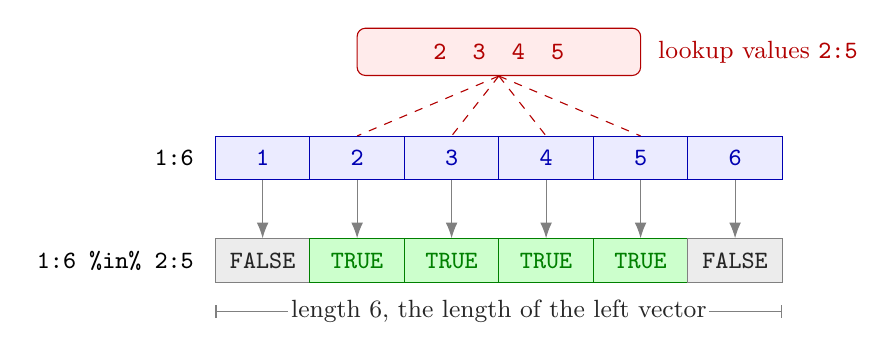
\begin{tikzpicture}[font=\small, >={Latex[length=2mm]},
  cell/.style={draw, minimum width=1.2cm, minimum height=0.55cm, inner sep=1pt, font=\small\ttfamily},
  val/.style={cell, draw=blue!70!black, fill=blue!8, text=blue!70!black},
  yes/.style={cell, draw=green!50!black, fill=green!20, text=green!50!black},
  no/.style={cell, draw=gray, fill=gray!15, text=gray!30!black},
  lab/.style={anchor=east, font=\small\ttfamily}]
  % lookup set
  \node[draw=red!70!black, fill=red!8, rounded corners=3pt, minimum height=0.6cm, minimum width=3.6cm,
        text=red!70!black, font=\small\ttfamily] (S) at (4.2,1.35) {2\quad 3\quad 4\quad 5};
  \node[anchor=west, red!70!black] at (6.1,1.35) {lookup values \texttt{2:5}};
  % left vector
  \node[lab] at (0.45,0) {1:6};
  \foreach \v [count=\i] in {1,2,3,4,5,6} { \node[val] (a\i) at (1.2*\i,0) {\v}; }
  \foreach \i in {2,3,4,5} { \draw[red!70!black, dashed] (S.south) -- (a\i.north); }
  % result
  \node[lab] at (0.45,-1.3) {1:6 \%in\% 2:5};
  \foreach \s/\t [count=\i] in {no/FALSE,yes/TRUE,yes/TRUE,yes/TRUE,yes/TRUE,no/FALSE} {
    \node[\s] (b\i) at (1.2*\i,-1.3) {\t};
    \draw[->, gray] (a\i.south) -- (b\i.north);
  }
  \draw[gray, |-|] (0.6,-1.95) -- (7.8,-1.95);
  \node[gray!30!black, fill=white, inner sep=1pt] at (4.2,-1.95) {length 6, the length of the left vector};
\end{tikzpicture}
\end{document}
